\apendice{Especificación de Requisitos}

Si procede.

\section{Descripción requisitos funcionales}

\begin{itemize}
    \item \textbf{RF-01 Iniciar sesión}: Todos los usuarios deben introducir de forma obligatoria su correo electrónico, tipo de usuario y contraseña para poder acceder a la página web.
    \item \textbf{RF-02 Consultar pacientes y usuarios}: Otorgar acceso a la lista completa de usuarios o pacientes, según los permisos asignados al usuario, y permitir la realización de búsquedas específicas dentro de ella.
    \item \textbf{RF-03 Gestionar pacientes y usuarios}: Permitir la creación y eliminación de cuentas, así como la modificación de los datos almacenados en las cuentas de pacientes y médicos. La capacidad para realizar estas acciones depende del nivel de acceso que el usuario tenga en el sistema web.
    \item \textbf{RF-04 Realizar actividad}: Ofrece las opciones de iniciar y finalizar actividades, así como la opción de guardar o descartar estas mismas. Existirá la posibilidad de realización de actividades sin que exista conexión entre el dispositivo físico y la página web, el denominado "modo offline".
    \item \textbf{RF-05 Mostrar actividades}: Presenta al usuario las actividades realizadas por el paciente, ya sea a través de un calendario de actividades o una lista con aquellas que cumplen unos criterios establecidos por el propio usuario.
    \item \textbf{RF-06 Consultar estadísticas}: Visualización de los datos relacionados con las actividades realizadas por el paciente, ya sea de una actividad en concreto o de todas en conjunto.
    \item \textbf{RF-07 Gestionar cuenta}: Facilitar a los usuarios las tareas de cambio de contraseña y actualización del correo eléctrónico vinculado a su cuenta.
    \item \textbf{RF-08 Cerrar sesión}: Todos los usuarios tendrán la opción de cerrar sesión desde el menú de inicio. Para prevenir cierres accidentales, se solicitará una confirmación de la acción antes de que esta se complete.
\end{itemize}


\section{Diagrama de casos de uso}


\begin{figure}[h]
    \centering
    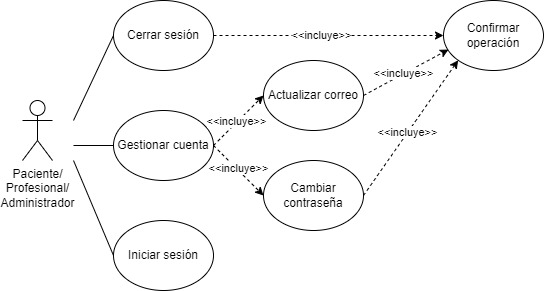
\includegraphics[width=1\textwidth]{img/CU-todos.jpg}
    \caption{CU-todos}
    \label{fig:CU-todos}
\end{figure}

\begin{figure}[h]
    \centering
    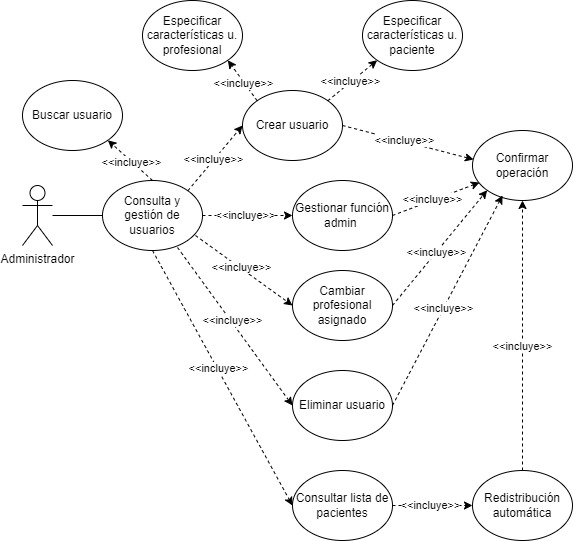
\includegraphics[width=1\textwidth]{img/CU-Administrador.jpg}
    \caption{CU-Administrador}
    \label{fig:CU-Administrador}
\end{figure}

\begin{figure}[h]
    \centering
    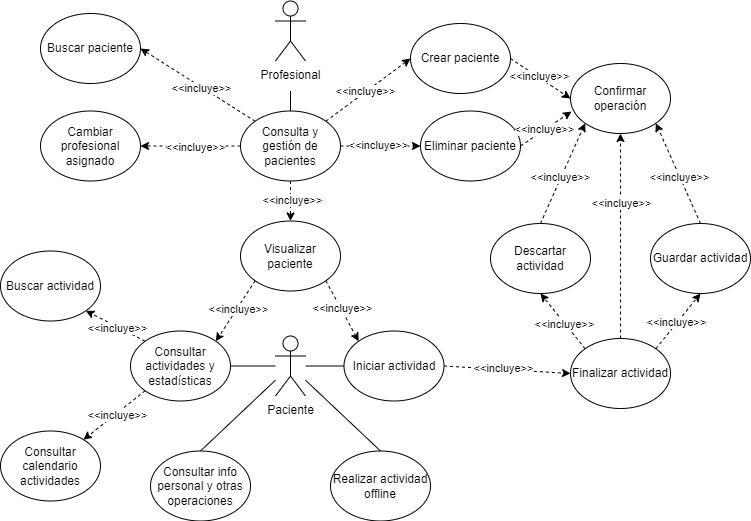
\includegraphics[width=1\textwidth]{img/CU-Paciente_Profesional.jpg}
    \caption{CU-Pacientes y Profesionales}
    \label{fig:CU-Paciente_Profesional}
\end{figure}




\section{Explicación casos de uso.}

Se puede describir mediante el uso de tablas o mediante lenguaje natural.    

Una muestra de cómo podría ser una tabla de casos de uso:

% Caso de Uso 1 -> Consultar Experimentos.
\begin{table}[p]
	\centering
	\begin{tabularx}{\linewidth}{ p{0.21\columnwidth} p{0.71\columnwidth} }
		\toprule
		\textbf{CU-1}    & \textbf{Ejemplo de caso de uso}\\
		\toprule
		\textbf{Versión}              & 1.0    \\
		\textbf{Autor}                & Alumno \\
		\textbf{Requisitos asociados} & RF-xx, RF-xx \\
		\textbf{Descripción}          & La descripción del CU \\
		\textbf{Precondición}         & Precondiciones (podría haber más de una) \\
		\textbf{Acciones}             &
		\begin{enumerate}
			\def\labelenumi{\arabic{enumi}.}
			\tightlist
			\item Pasos del CU
			\item Pasos del CU (añadir tantos como sean necesarios)
		\end{enumerate}\\
		\textbf{Postcondición}        & Postcondiciones (podría haber más de una) \\
		\textbf{Excepciones}          & Excepciones \\
		\textbf{Importancia}          & Alta o Media o Baja... \\
		\bottomrule
	\end{tabularx}
	\caption{CU-1 Nombre del caso de uso.}
\end{table}

\section{Prototipos de interfaz o interacción con el proyecto.}


